\section{Deelvraag 4: Requirements}
In dit hoofdstuk word de vierde deelvraag onderzocht \SubquestionFour.
Om met deze deelvraag te beantwoorden zijn er semi gestructureerde interviews gehouden met de product owner en de CEO van Snakeware.
Tijdens de interviews wordt er gepraat over de eisen en wensen zodat deze in kaart kunnen worden gebracht.
Bijde interviews zijn terug te vinden in bijlage \ref{appendix:ExploreUserRequirements}

\subsection{Interviews met sleutelfiguren}
Het eerste interview wat plaats heeft gevonden is gedaan met de product owner Elsa Croes.
Om Elsa te ondersteunen en meer technisch kennis mee te nemen in het interview is er op het laatst een frontend developer mee genomen in het gesprek Eric Dijkstra.
Het interview heeft plaats gevonden op 6 november 2023 op locatie.
Tijdens het interview zijn er verschillende vragen gesteld om een beeld te krijgen van de toekomst visie van de applicatie.
Het complete interview is te vinden in bijlage \ref{appendix:ExploreUserRequirementsElsa}.

\whitespace
Daarnaast is er ook interview gedaan met de CEO van Snakeware Hans Hoomans.
Het interview heeft plaats gevonden op 7 november 2023 op locatie.
Tijdens het interview met hans zijn we heel erg van de orgineele vragen af gegaan. 
Aan het einde van het interview zijn we de vragen nog een keer langs gelopen en hebben we hier uit verschillende requirements gehaald.
Omdat dit interview niet als transcriptie gebruikt kan worden is er een samenvatting gemaakt en is te vinden in bijlage \ref{appendix:ExploreUserRequirementsHans}.

% De complete lijst met de requirements die uit dit interview zijn te zien in \ref{fig:ElsaRequirements}.
%
% \whitespace
% \begin{graphic}
%     \captionsetup{type=figure}
%     \caption{Elsa Croes Requirements}
%     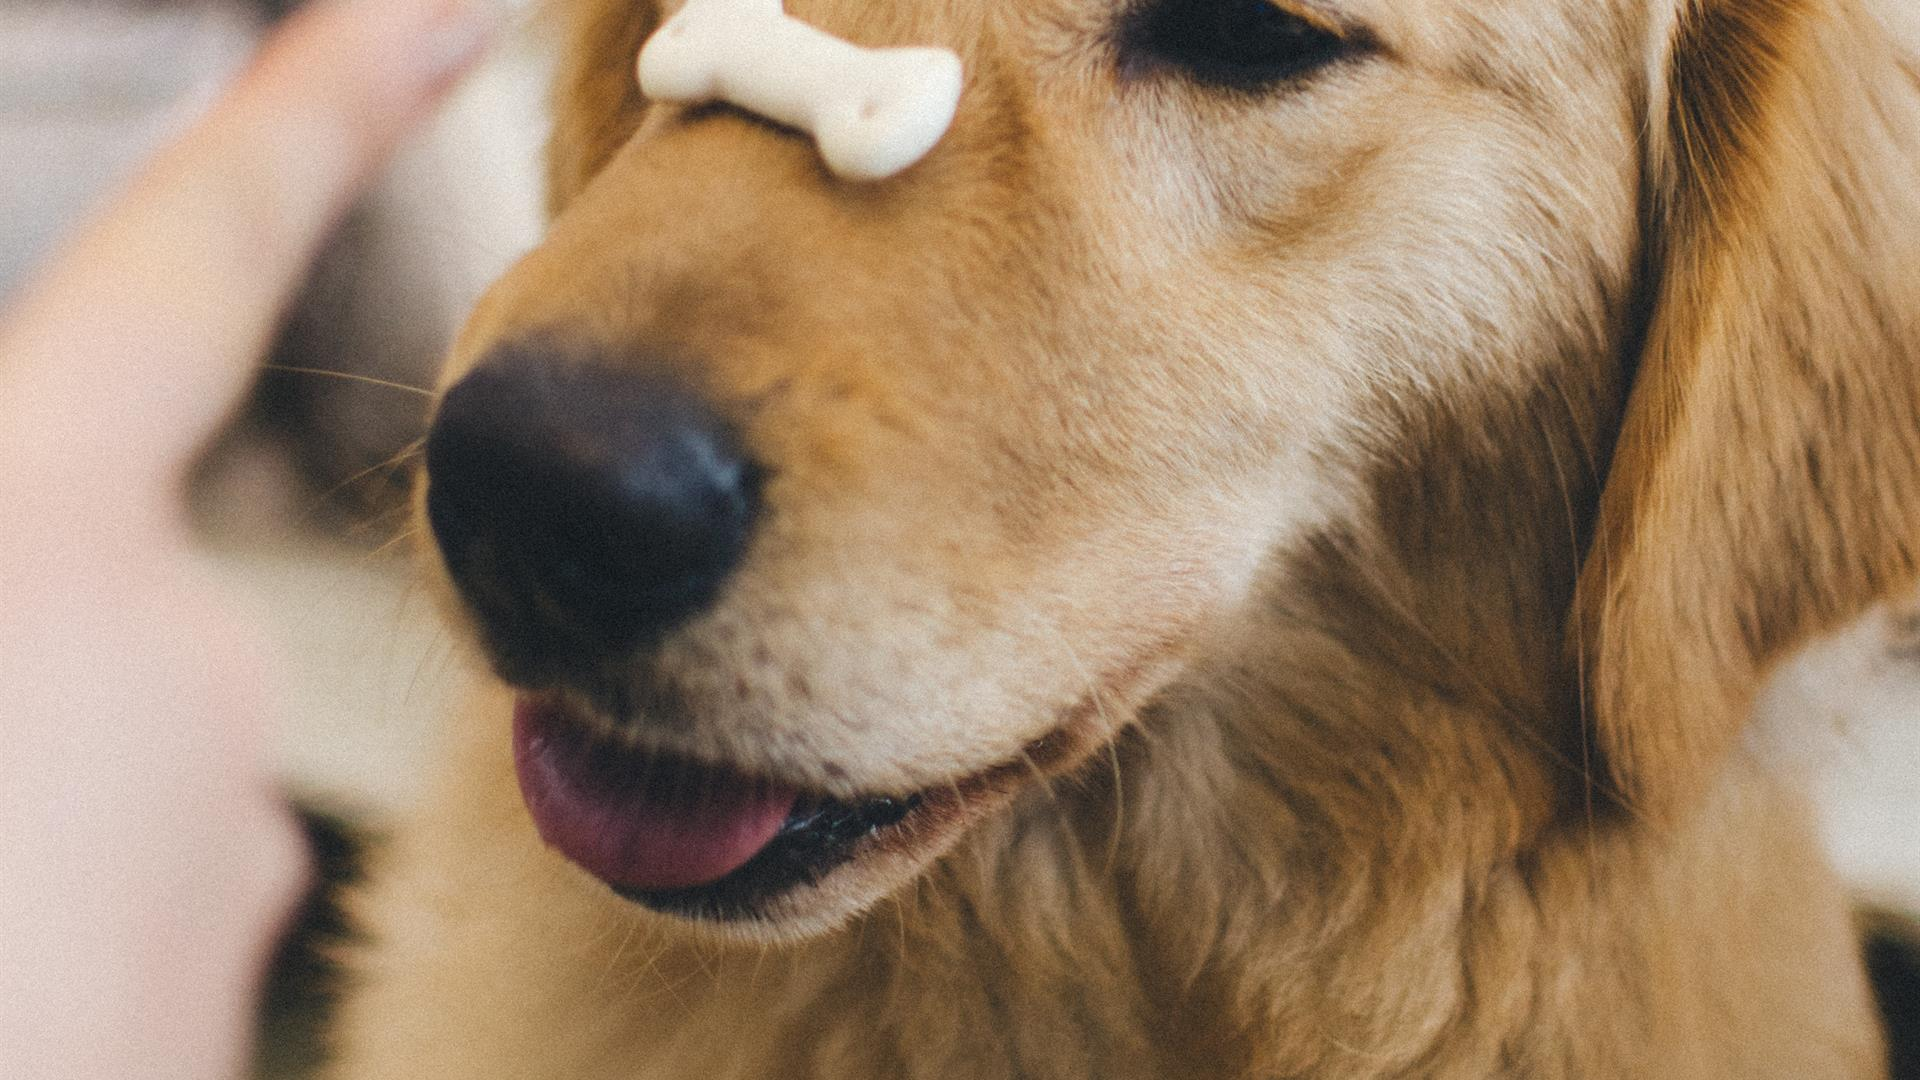
\includegraphics[scale=0.2]{Placeholder.jpg}
%     \label{fig:ElsaRequirements}
% \end{graphic}

\subsection{Antwoord en resultaat}
Na dat beide interviews waren afgenomen is er een lijst van user stories gemaakt.
Deze user stories zijn beide door Hans en Elsa als correct beschouwd.
in figuur \ref{fig:RequirementSimplified} zij de requirements te vinden.

% Het andere interview is gedaan met de CEO van Snakeware Hans Hoomans.
% De complete transcriptie van het interview is te vinden in bijlage \ref{appendix:ExploreUserRequirementsHans}
% Het interview heeft plaats gevonden op 7 november 2023 op locatie.
%



\begin{graphic}
    \captionsetup{type=figure}
    \caption{Hans Hoomans Requirements}
    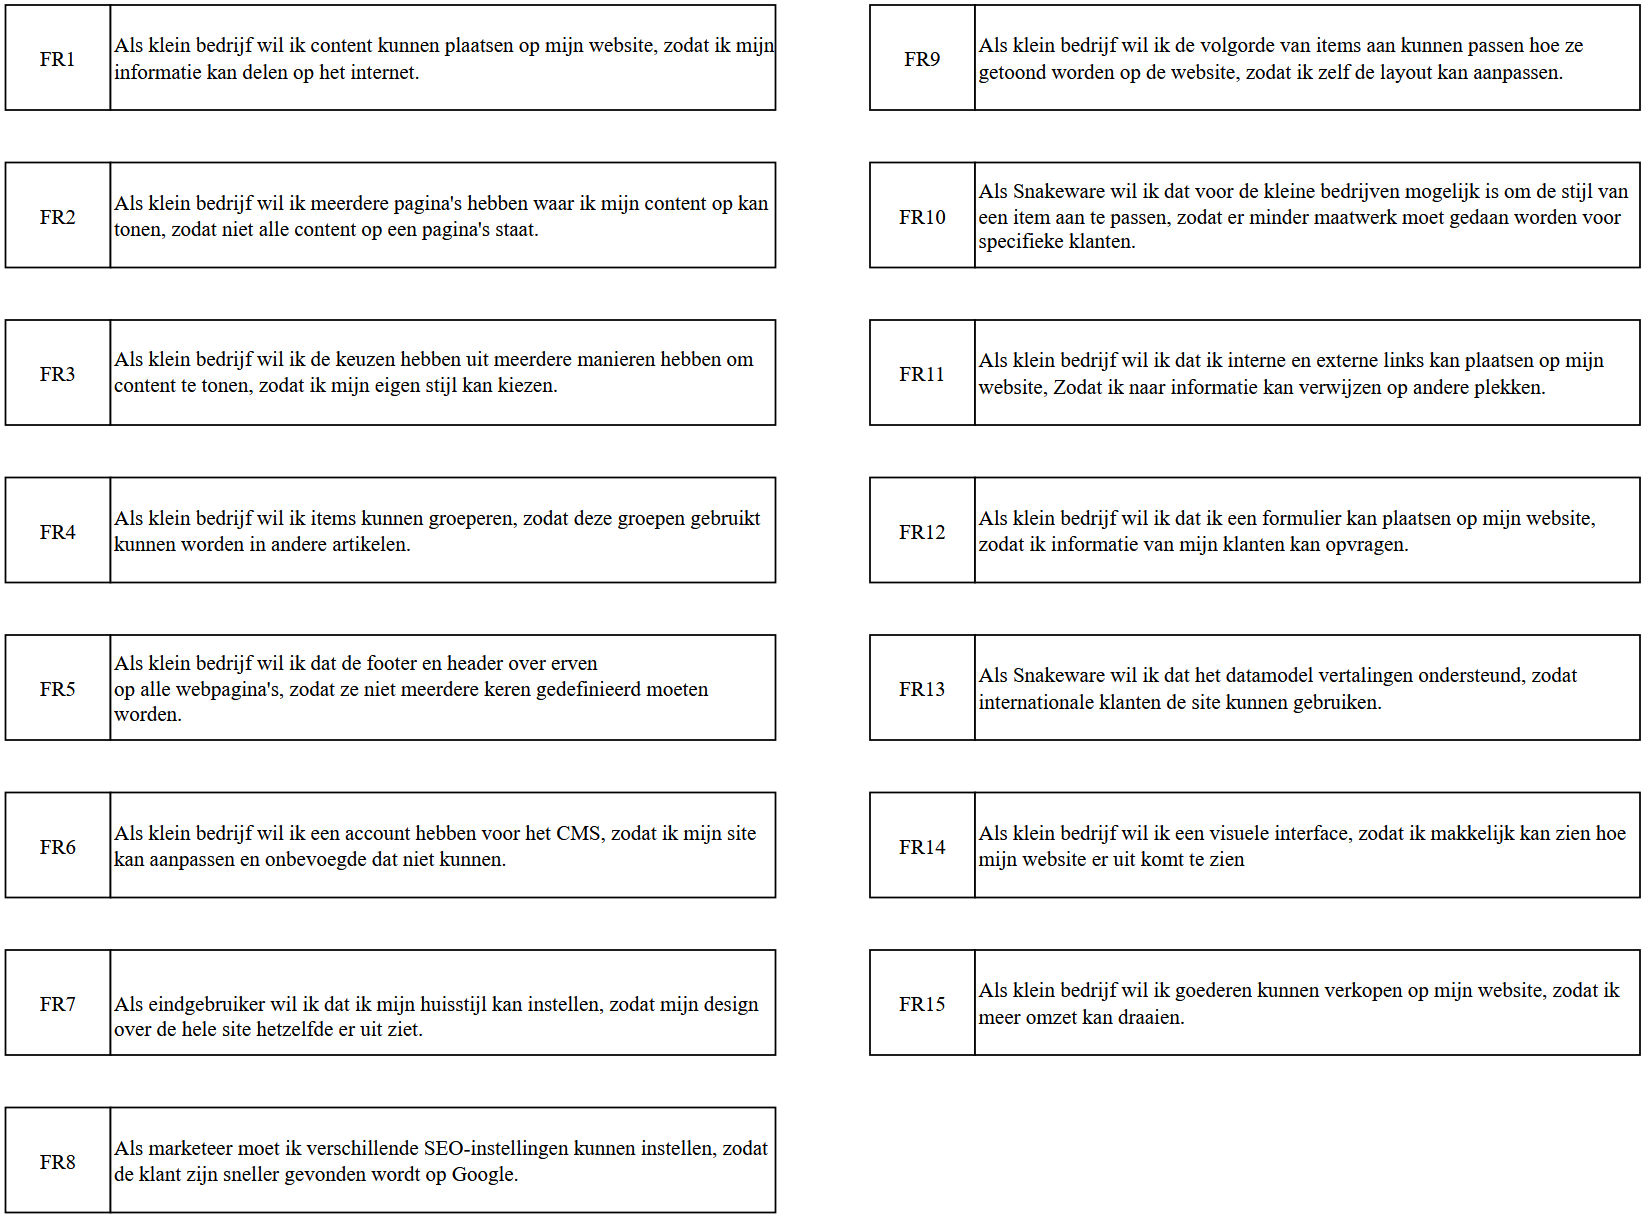
\includegraphics[scale=0.8]{Requirements}
    \label{fig:RequirementSimplified}
\end{graphic}
